\chapter{Branching ratio}
To measure the inclusive branching fractions

\begin{equation}
    Br(B^{+/-} \rightarrow \Lambda_c^{+} X) = \frac{ N_{tag, \Lambda_c} \cdot  \epsilon^{+}_{FEI}}{N_{tag} \cdot Br(\Lambda_c^+ \rightarrow  p K^- \pi^+) \epsilon_{\Lambda_c} \epsilon^{+}_{FEI,  sig }}
\end{equation}\label{eq:chargedB_BRformula}

\begin{equation}
    Br(B^{0} \rightarrow \Lambda_c^{+/-} X) = \frac{ N_{tag, \Lambda_c} \cdot  \epsilon^{0}_{FEI}}{N_{tag} \cdot Br(\Lambda_c^+ \rightarrow  p K^- \pi^+) \epsilon_{\Lambda_c} \epsilon^{0}_{FEI,  sig }}
\end{equation}\label{eq:B0_BRformula}

the following quantities need to be known: 
\begin{itemize}

\item $N_{tag, \Lambda_c} $ is the reconstructed signal yield obtained from a two dimensional fit of $M_{bc}$ and $M(p K \pi)$ in the final sample.
\item ${N_{tag}}$ is the reconstructed signal yield obtained from the $M_{bc}$ fit of all the tagged $B$ mesons in the final sample.
\item $\epsilon_{\Lambda_c} $ is the $\Lambda_c$ reconstruction efficiency.
\item $\epsilon^{+}_{FEI}$ ($\epsilon^{0}_{FEI}$) represent the hadronic tag-side efficiency for generic $B^+B^- $ ($B^0\bar{B^0}$) events. 
\item $\epsilon^{+}_{FEI,  sig}$ ($\epsilon^{0}_{FEI,  sig }$) represents the hadronic tag-side efficiency for  $B^+B^-$ ($B^0\bar{B^0}$) events where the tagged $B$ meson decays hadronically and the accompanying meson decays inclusively into the studied signal channel. 
\item  $Br(\Lambda_c^+ \rightarrow  p K^- \pi^+) $: the branching fraction of the decay mode used to reconstruct the  $\Lambda_c$ baryon.
\end{itemize}
\vspace{0.2 cm}


\begin{table}[H]
    \centering
    \resizebox{0.95\textwidth}{!}{%
    \setlength{\tabcolsep}{8pt}
    \begin{tabular}{c c c c c c c}
    
    \toprule
     \hline
         &  total fit \hspace{0.5 cm}  & signal fit  &  BELLE MC VALUE  \\
     \midrule
     \hline
    stream 0	&	(2.84 $\pm$ 0.13)$\%$  &	(2.96 $\pm$ 0.07)$\%$	 &	(2.91 $\pm$ 0.03)$\%$\\
    stream 1	&	(2.82 $\pm$ 0.14)$\%$	&	(2.99 $\pm$ 0.07)$\%$	 &	(2.91 $\pm$ 0.03)$\%$	\\
    stream 2	&	(2.97 $\pm$ 0.14)$\%$	&	(2.97 $\pm$ 0.07)$\%$	 &	(2.90 $\pm$ 0.03)$\%$\\
    stream 3	&	(2.76 $\pm$ 0.14)$\%$	&	(2.90 $\pm$ 0.07)$\%$	 &	(2.91 $\pm$ 0.03)$\%$\\
    stream 4	&	(3.06 $\pm$ 0.14)$\%$ &	    (3.05 $\pm$ 0.07)$\%$	 &	(2.90 $\pm$ 0.03)$\%$\\
    stream 5	&	(2.83 $\pm$ 0.14)$\%$	&	(2.84 $\pm$ 0.07)$\%$	 &	(2.92 $\pm$ 0.03)$\%$\\
    \midrule
    \hline
    average			&	(2.88 $\pm$	0.06)$\%$	&	(2.95 $\pm$	0.03)$\%$	& (2.91 $\pm$ 0.01)$\%$\\
    \bottomrule
    \hline
    \end{tabular}%
    }
    \label{tab:SixStreams_chargedCorrLamBR}
    \caption{charged corr}
    %\caption{Measured branching fraction values obtained using the results listed in \cref{tab:SixStreams_chargedCorrLam2Dfits} for the six different streams (only statistical uncertainties are displayed) and its average.}
    \end{table}

    \begin{table}[H]
        \centering
        \resizebox{0.95\textwidth}{!}{%
        \setlength{\tabcolsep}{8pt}
        \begin{tabular}{c c c c c c c}
        
        \toprule
         \hline
             &  total fit \hspace{0.5 cm}  & signal fit  &  BELLE MC VALUE  \\
         \midrule
         \hline
        stream 0	&	(1.24 $\pm$ 0.11)$\%$  &	(1.19 $\pm$ 0.05)$\%$	 &	(1.217 $\pm$ 0.002)$\%$\\
        stream 1	&	(1.24 $\pm$ 0.11)$\%$	&	(1.21 $\pm$ 0.05)$\%$	 &	(1.218 $\pm$ 0.002)$\%$	\\
        stream 2	&	(1.35 $\pm$ 0.12)$\%$	&	(1.23 $\pm$ 0.05)$\%$	 &	(1.218 $\pm$ 0.002)$\%$\\
        stream 3	&	(1.16 $\pm$ 0.10)$\%$	&	(0.20 $\pm$ 0.05)$\%$	 &	(1.215 $\pm$ 0.002)$\%$\\
        stream 4	&	(1.44 $\pm$ 0.13)$\%$   &	(1.21 $\pm$ 0.05)$\%$	 &	(1.218 $\pm$ 0.002)$\%$\\
        stream 5	&	(1.04 $\pm$ 0.11)$\%$	&	(1.15 $\pm$ 0.05)$\%$	 &	(1.217 $\pm$ 0.002)$\%$\\
        \midrule
        \hline
        average		&	(1.25 $\pm$	0.05)$\%$	&	(1.20 $\pm$	0.02)$\%$	& (1.217 $\pm$ 0.001)$\%$\\
        \bottomrule
        \hline
        \end{tabular}%
        }
    \label{tab:SixStreams_chargedAntiCorrLamBR}
    \caption{charged anticorr}
    %\caption{Measured branching fraction values obtained using the results listed in \cref{tab:SixStreams_chargedCorrLam2Dfits} for the six different streams (only statistical uncertainties are displayed) and its average.}
    \end{table}

\section{Systematics}


\subsection{Continuum background}\label{sec:continuumSysBtoLambdaC}

2 sources of systematics:
\begin{itemize}
\item difference in the shapes 
\item different impact of the Continuum Suppression cut
\end{itemize}

To estimate the first type of uncertainty two-dimensional fits with varied parameters' values by their uncertainties 
(a fit with $+$err and $-$err) were performed. \\
The rescaling procedure used to model the on-resonance continuum distribution is far from perfect, especially in the case of the $B_{tag}$ fit.
As one can see from \cref{fig:stream5_chargedBtag_Total_fit}:
\\
\begin{figure}[H]
    \centering
    \subcaptionbox{\label{fig:stream5_chargedBtag_Total_fit}}
    {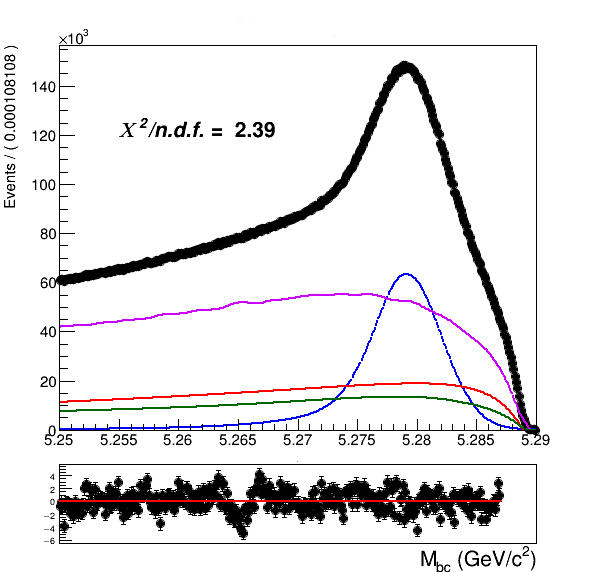
\includegraphics[width=.65\textwidth]{07-LamBR/figs/stream5_chargedBtag_Total_fit.png}} 
    \subcaptionbox{\label{fig:stream5_chargedBtag_TotalFit_TrueContinuum}}
    {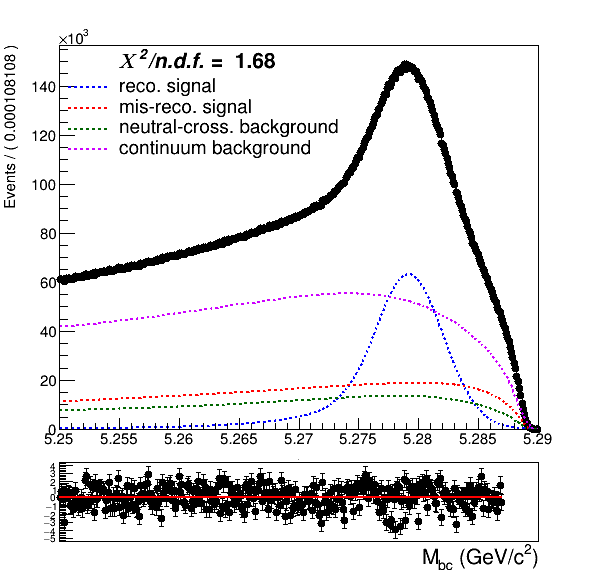
\includegraphics[width=.65\textwidth]{07-LamBR/figs/NEW_stream5_chargedBtag_Total_fit_sigmaCB_misReco_Tail_free_usingTrueContinuumPDF_370bins.png}} 
    \caption{Above: Fitted $M_{bc}$ of charged correlated decays with scaled off-resonance continuum distribution. 
    Below: same $M_{bc}$ distribution with the true continuum distribution.}
    \end{figure}
  
The bumps visible for  $M_{bc} < 5.27 GeV/c^2$ in \cref{fig:stream5_chargedBtag_Total_fit}   
are a consequence of the imperfect scaling procedure used to model the continuum background. In fact, 
they disappear completely (in \cref{fig:stream5_chargedBtag_TotalFit_TrueContinuum} ) when the same fit is performed using 
the pdf obtained directly from the on-resonance distribution (\cref{fig:stream5_chargedBtag_continuumHistPdf})
There is a significant impact on the fit results, the values from the  $B_{tag}$ fit in the charged correlated channel are reported here below:

\begin{table}[H]
    \begin{tabular}{ |p{2.5cm}||p{4.5cm}| p{4.5cm}| }
    \hline
        \    &  Fit with scaled continuum &  Fit with true continuum\\
     \hline
     $N_{recSig}$  yields     &  $4.7787  \cdot 10^6 \pm 6.75 \cdot 10^3 $   & $ 4.7474  \cdot 10^6 \pm 8.01 \cdot 10^3$\\
   
     \hline
    \end{tabular}
    \caption{Signal yields obtained in $B_{tag}$ fits shown in \cref{fig:stream5_chargedBtag_Total_fit} and \cref{fig:stream5_chargedBtag_TotalFit_TrueContinuum}.}
    \end{table}
    \vspace{0.2 cm}

The yields are to be compared with the values obtained when fitting the total signal distribution shown
in \cref{fig:chargedBtag_corrLambdaC_TotalSignalBtag_fit}: $N_{recSig} = 4.7571  \cdot 10^6 \pm 3.23 \cdot 10^3$.
The continuum modeling alone is responsible for a discrepancy of about 3.2$\sigma$ on the yields.
This discrepancy and the impact on the branching fraction are accounted in the systematic uncertainties derived from the continuum modeling. 
This source of systematics is responsible for 0.02 $\%$ uncertainty on the branching ratio.
\begin{figure}
    \centering
    {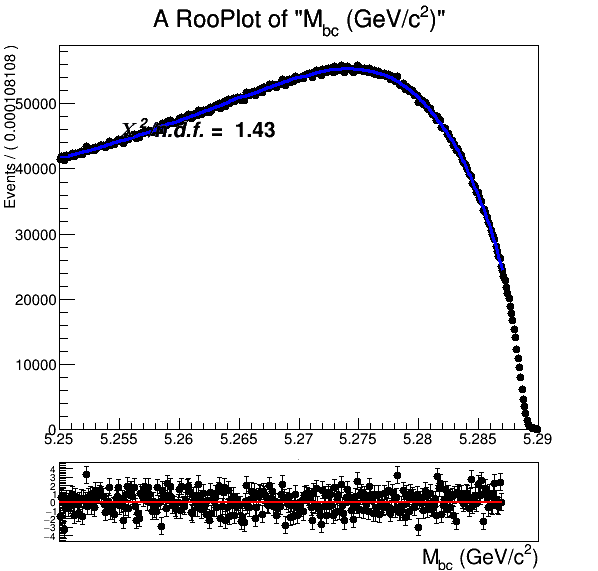
\includegraphics[width=0.5\textwidth]{07-LamBR/figs/stream5_chargedBtag_continuumHistPdf.png}}
    \caption{$M_{bc}$ on-resonance MC distribution of charged correlated decays.}
    \label{fig:stream5_chargedBtag_continuumHistPdf}
    \end{figure}
The other type of systematic uncertainty in modeling the continuum is originated by the continuum suppression cut having a slightly different efficiency on data (as a consequence of the shift in off-resonance MC and data visible in the the $foxWolframR2$ distribution in Fig. \ref{fig:R2_MC-Data_off_resonance_distributions}). 
As already discussed, it originates a possible  discrepancy of about 2.25$\%$ in continuum background events in the two dimensional fit (and only 1.25$\%$  in the $B_{tag}$ fit). The statistical uncertainty on this fraction of events can also be taken into account as systematics. 
Being the number of events in the off-resonance data sample without the continuum suppression applied is very small, the uncertainty in the mentioned fraction of events is negligible compared to the statistical uncertainty on the on-resonance continuum background events in MC: it would account for 0.002$\%$ on the BR value. 
Therefore, this second source of uncertainty is not taken into account.
There would be also a third of systematic uncertainty given by potential difference in the on-/off-resonance correction between data and MC, but there's no way one can estimate it properly.


\subsection{Crossfeed ratio}\label{sec:CrossfeedRatioSysBtoLambdaC}
The ratio crossfeed/misreconstructed signal is kept fixed in the $B_{tag}$ fit to the MC value.
 This choice was made according to the fact that the two categories of events have  
a similar origin: in both cases the $B$ mesons were not correctly reconstructed, either because of missing or wrongly added particles 
(misreconstructed signal events) or, in the case of crossfeed events because the tagged $B$ meson was not the required
 one ($B^0$ meson instead of a $B^{+/-}$ meson). 
The ratio between these two categories of events is therefore expected to be very similar in MC and data, 
though there's no guarantee that the efficiency to reconstruct them is the same in data in data and consequently 
the above mentioned ratios could differ on data. Unfortunately there's no direct way to have an estimate of the possible 
discrepancy for them.\\  
In \cite{gelb_moritz_2018_21546} (and previously in \cite{schwab_judith_2017_21422}) it was found that there's a substantial 
difference in terms of tagging efficiency for FEI applied on Monte Carlo and on Belle data, being the discrepancy around $\sim$ 20$\%$. 
We can assume that the efficiency for the two categories of events on data will both differ of that value and the ratio of the events 
being the same MC value, but in absence of any other method to estimate the uncertainty on it one can consider a maximal 
discrepancy of 20$\%$ between Monte Carlo and data to study the impact on the yields\footnote{This method was also validated 
with the control decay sample and the originated uncertainty is well within the PDG reported ones.}. 

\subsection{Crossfeed $B_{tag}$ PDF}
Since also the shapes of the PDFs decribing the crossfeed background in the $B_{tag}$ fit are fully fixed to the
ones determined with the limited Monte Carlo statistics, also their statistical uncertainties
need to be taken into account as possible source of systematics.
To estimate this source of uncertainty fits with varied parameters' values by their uncertainties 
(a fit with $+$err and $-$err) were performed.

\subsection{2DFit crossfeed normalization}
As discussed in the 2D simulateous fit section, in each decay channel the normalization of crossfeed events 
is estimated using the fitted reconstructed signal events of the corresponding crossfeeding channel in the as follows:
\begin{equation}
N_{cross } = N_{recSig}^{correlated} (\dfrac{\epsilon_{cross}}{\epsilon_{recSig}})^{correlated} + 
N_{recSig}^{anticorrelated} (\frac{\epsilon_{cross}}{\epsilon_{recSig}})^{anticorrelated}
\end{equation}
where  $\epsilon_{recSig}$  and $\epsilon_{cross}$ are respectively the efficiency to reconstruct correctly
 signal events in the crossfeeding channel and the efficiency of reconstructing those events as crossfeed in the
 channel of interest.\\
 The uncertainties of those two efficiencies may cause an overestimation or underestimation of the crossfeed 
 in the channel of interest. To estimate the systematic uncertainty deriving from it, the simultaneous fits 
 have been performed modifying the ratio of the efficiencies by the respective uncertainties maximising the shift, 
 i.e. using $\frac{\epsilon_{cross} + \sigma}{\epsilon_{recSig} - \sigma}$ and $\frac{\epsilon_{cross} - \sigma}{\epsilon_{recSig} + \sigma}$ 

 \subsection{2DFit $M_{bc}$ peaking/flat PDFs}
As discussed in \cref{sec:MC2D_Fit} the shapes of the PDFs describing the generic background (peaking or flat in $M_{bc}$ ) are kept fixed
 in the two dimensional fit. This source of systematics is handled in the same way as the crossfeed background in the $B_{tag}$:
 fits with varied parameters' values by their uncertainties were performed (procedure is repeated for $M_{bc}$ peaking and flat background).

 \subsection{PID  efficiency correction}\label{sec:chargedCorrPIDcorrSys}

 The PID selection efficiency for the three charged particles in the signal decay needs
 to be corrected on MC due to various differences, when comparing to data. The
 Belle PID group has prepared a set of correction factors and tables of systematic
 uncertainties for PID efficiencies for all charged particles.
 %The PID efficiency in data is usually lower in data than in Monte Carlo simulations, therefore the efficiency of reconstructing $\Lambda_c$ baryons needs to be corrected accordingly when calculating the branching fraction on data, taking into account the PID corrections corresponding to each of the hadrons in which it decays\footnote{since on all of them a PID selection cut is applied}. \\
 The proton identification efficiency was studied in \cite{PIDeff}.
 The inclusive $\Lambda^0$ decay $\Lambda^0 \rightarrow p \pi^-$   was used to examine the proton identification efficiency difference between data 
 and MC in \textit{Belle}. The datasets for the SVD1 and SVD2 periods are treated separately, and the efficiency ratio dependence on proton charge, 
 momentum and polar angle is considered. The study is done for the proton ID cut values 0.6, 0.7, 0.8 and 0.9\footnote{Here, proton ID cut value $X$ means $  \mathcal{L}_{p/K} > X$ and $  \mathcal{L}_{p/\pi} > X$}. 
 The binning on the momentum starts at 0.2 GeV. 
 The proton ID efficiency is defined as\\
 \vspace{0.2cm}
 \newline
 \hspace{3 cm}    $\epsilon_{PID} = \frac{\text{number of}\hspace{0.05 cm}p \text{tracks identified as} \hspace{0.05 cm} p}{\text{number of }p \hspace{0.05 cm} \text{tracks} }$\\
 
 \vspace{0.2cm}
  and the comparison between MC efficiency and data efficiency by a double ratio defined as \\
 
 \vspace{0.2cm} \hspace{1 cm}  $ R_p = \epsilon^{data}/\epsilon^{MC}$ \\
 
 \vspace{0.5cm}
 \noindent The average proton ID correction is estimated to be: \hspace{0.5 cm} $R_p = 0.969 \pm 0.003$.
 
 \vspace{0.2 cm}
 \noindent  The kaon identification efficiency was studied in detail in Belle Note 779 \cite{KIDeff} (\url{http://belle.kek.jp/secured/belle_note/gn779/bn779.ps.gz}). The decay $D^{*+} \rightarrow D^0 \pi^+$ followed by $D^0 \rightarrow K^- \pi^+$, was used to examine it. As for the proton identification efficiency it considers the dependence on Kaon charge, momentum and polar angle and same ID cut values\footnote{Here, Kaon ID cut value $X$ means $  \mathcal{L}_{K/\pi} > X$, so for values below $X$ the tracks are identified as pions} 

\subsection{$B^- \rightarrow \Lambda_c^+$ decays}
Regarding the systematic uncertainties deriving from the continuum modeling in the two-dimensional fit are estimated as 
already described in \ref{continuumSysBtoLambdaC} one obtains an absolute value of $0.04\%$ on the branching fraction.\\
Instead the imperfect modeling of the continuum in the $B_{tag}  $ fit is responsible for a 0.02 $\%$ on the branching fraction in absolute value.\\
Continuum modeling uncertainties account for 0.05$\%$ total uncertainties on the branching fraction in absolute value.
\vspace{1 cm}

To estimate the systematics derived from the crossfeed/misreconstructed signal ratio, in the $B_{tag}$ fit the number of crossfeed events 
were varied artificially in order to have $\pm$20$\%$ different ratio, keeping the previosuly determined Monte Carlo ratio fixed.

\vspace{0.25 cm}
\begin{table}[H]
\begin{tabular}{ |p{2.5cm}||p{2cm}| p{2cm}|  p{2cm}|}
\hline
       &  $- \sigma$ &  $+ \sigma$ & $ \pm \bar{\sigma}$\\
 \hline
 offset    &  20010 &  9330 & 14670 \\
 \hline
\end{tabular}
\caption{Offsets on the $N_{recSig}$  signal yields obtained varying of $\pm$20$\%$ the 
 ratio of crossfeed/misreconstructed events in the $B_{tag}$ fit and mean deviations reported in the last column.}
\end{table}

The offsets that a potential $\pm$20$\%$ different crossfeed/misreconstructed signal ratio produce results in 0.01$\%$ systematic
uncertainity on the branching fraction.
\\
The systematic uncertainties deriving from the crossfeed background modeling in the $B_{tag}$ fit is estimated following 
the same procedure  described for continuum modeling systematics in the two dimensional fit.\\
In the table below the signal yields' offsets are listed changing
the parameters within their uncertainties, and the mean offsets value used to calculate the
expected uncertainty on the BR value. The resulting absolute systematic uncertainty is
about 0.01$\%$ on the BR value.
\vspace{0.25 cm}
\begin{table}[H]
\begin{tabular}{ |p{2.5cm}||p{2cm}| p{2cm}|  p{2cm}|}
\hline
       &  $- \sigma$ &  $+ \sigma$ & $ \pm \bar{\sigma}$\\
 \hline
 offset    &  14810 &  17280 & 16045 \\
 \hline
\end{tabular}
\caption{Offsets on the $N_{recSig}$  signal yields  obtained varying the parameters of crossfeed
background PDFs within their uncertainties in the $B_{tag}$ fit and mean
deviations reported in the last column. }
\end{table}

\begin{table}[h]
    \centering
    \resizebox{0.8\textwidth}{!}{%
    \begin{tabular}{c c c}
    \hline
    source              & relative ($\%$) & absolute ($\%$)  \\
    \hline
    Continuum modeling   &  1.77   &  0.05 \\
    $B_{tag}$ fit Crossfeed fraction   &  0.35 &  0.01 \\
    $B_{tag}$ fit Crossfeed PDF shape & 0.35 &  0.01  \\
    2DFit crossfeed normalization & 0.70 & 0.02 \\
    $M_{bc}$ peaking PDF shape & 0.35 &  0.01  \\
    $M_{bc}$ flat PDF shape & 0.35 &  0.01 \\
    
    $\epsilon^{+}_{FEI,  sig}/\epsilon^{+}_{FEI}$ & 0.35 & 0.01 \\
    $\epsilon_{\Lambda_c}$ & 1.41 & 0.04 \\
    PID            & 1.75    & 0.05 \\
    Tracking efficiency & 0.35  & 0.01 \\
    \hline
    Total                         &   3.18     &  0.09  \\
    \hline
    \end{tabular}%
    }%
    \caption{Systematic uncertainties in the determination of the  $B^+ \rightarrow \bar{\Lambda}_c^- X$ branching fraction in \si{\percent}.}
    \label{tab:systematics:ChargedCorr}
    \end{table}
    

    \subsection{$B^+ \rightarrow \Lambda_c^+$ decays}

    Regarding the systematic uncertainties deriving from the continuum modeling in the two-dimensional fit are estimated 
    one obtains an absolute value of $0.02\%$ on the branching fraction.\\